\section{Semantic Segmentation}

\todo[inline, color=red!50]{Add topic: Metrics (accuracy etc.)}

Semantic segmentation involves identifying pixels in images that belong to a specific class,
sometimes identifying pixels to belong to a specific instance of a class. It can be seen as supervised learning at the pixel level.

\begin{figure}[h]
	\centering
	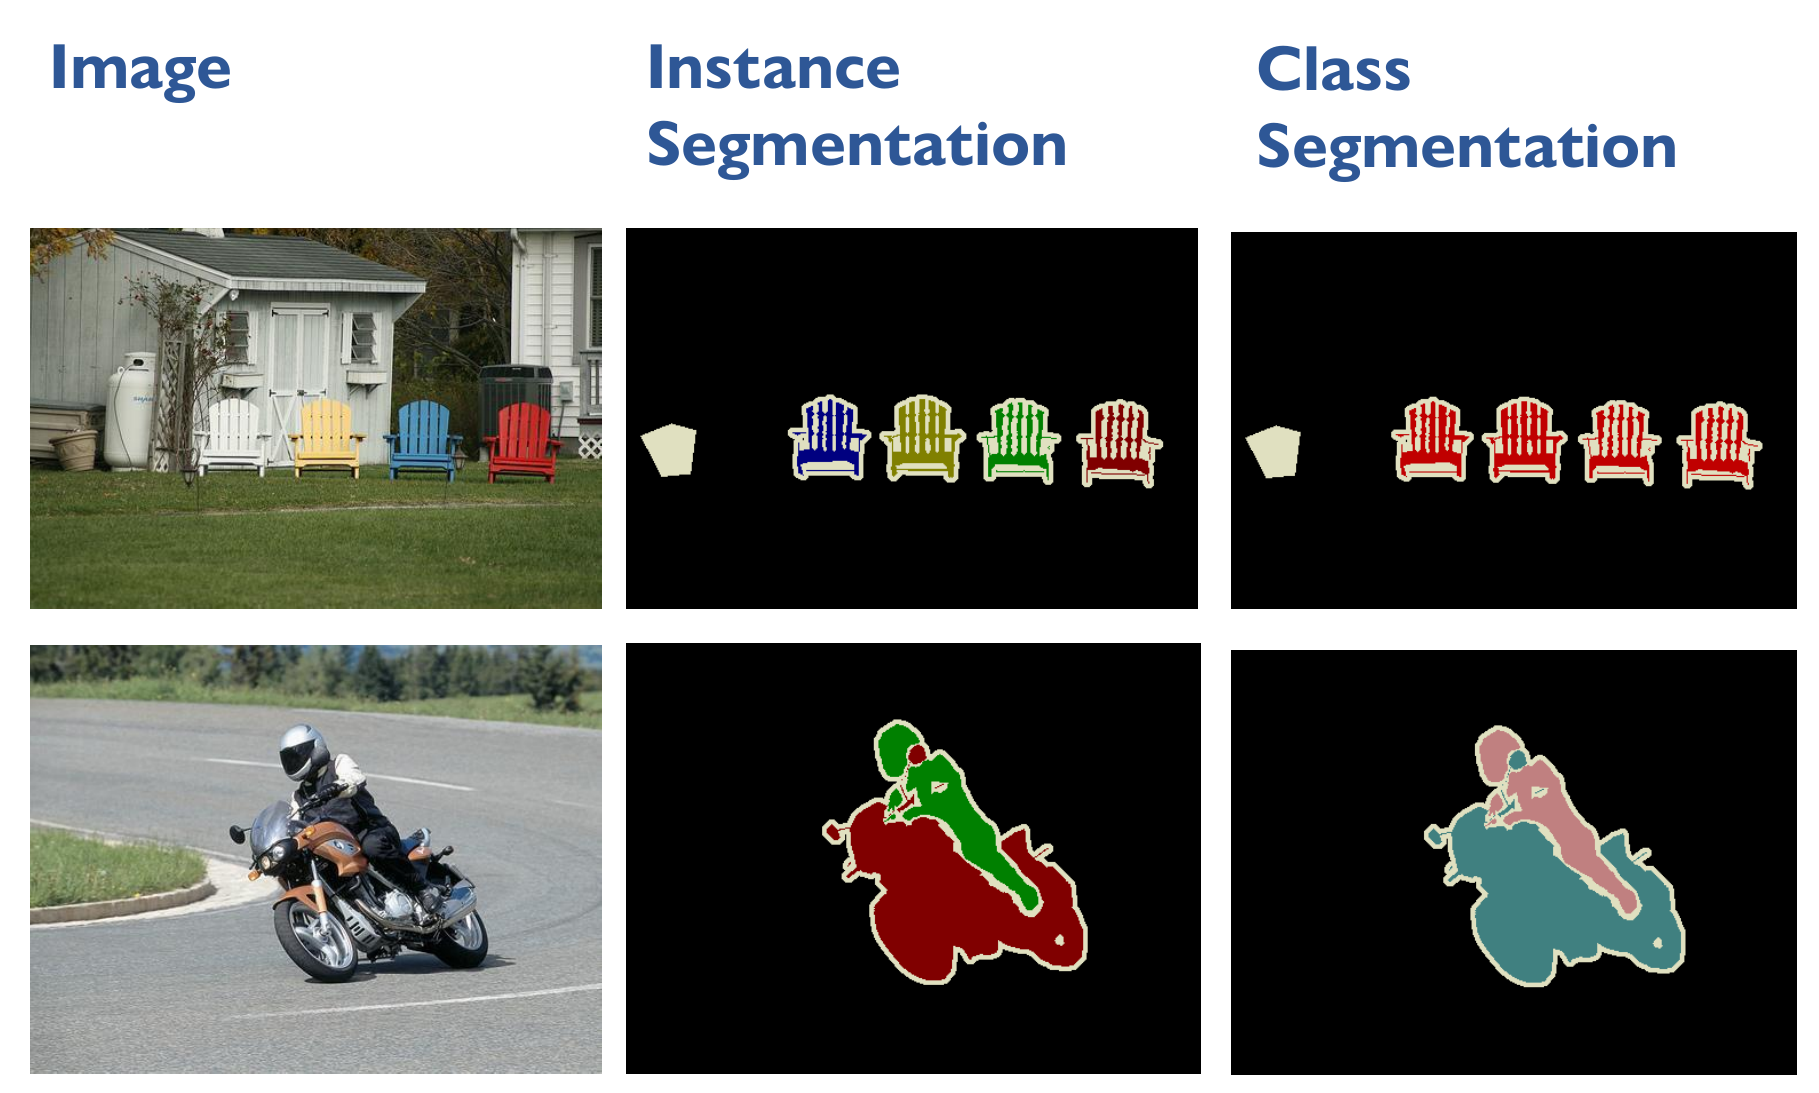
\includegraphics[width=0.7\linewidth]{img/semantic_segmentation}
	\caption{Semantic Segmentation Example}
\end{figure}

Non-semantic segmentation aims to find regions in images without additional information like classes.
It is similar to unsupervised learning and often follows a bottom-up approach.
Segmentation, in general, seeks a compact representation of a scene in terms of regions that share common properties.

\subsection{k-Means Clustering}

K-Means clustering is not an optimal solution for image clustering. Lloyd's algorithm is one possibility for clustering with the following steps:

\begin{itemize}
	\item Initialize cluster centers (e.g., randomly).
	\item Assign samples to clusters.
	\item Calculate mean values of clusters as new centers.
	\item Iterate until clusters don't change.
\end{itemize}

Issues with K-Means include the requirement to specify the number of clusters and the assumption of spherical cluster shapes.

\subsection{Mean Shift Clustering}

Mean Shift clustering allows variable cluster shapes, avoiding the need for predefined shapes. The algorithm involves:

\begin{enumerate}
	\item Search for the maximum of the feature density from a given position in the image.
	\item Define a cluster as the set of positions that converge to the same maximum.
\end{enumerate}

The algorithm deals with the challenge of searching for local maxima by using Kernel Density Estimation with a Gaussian kernel
or the Derivative of the Gaussian for direct approximation.

\begin{figure}[h]
	\centering
	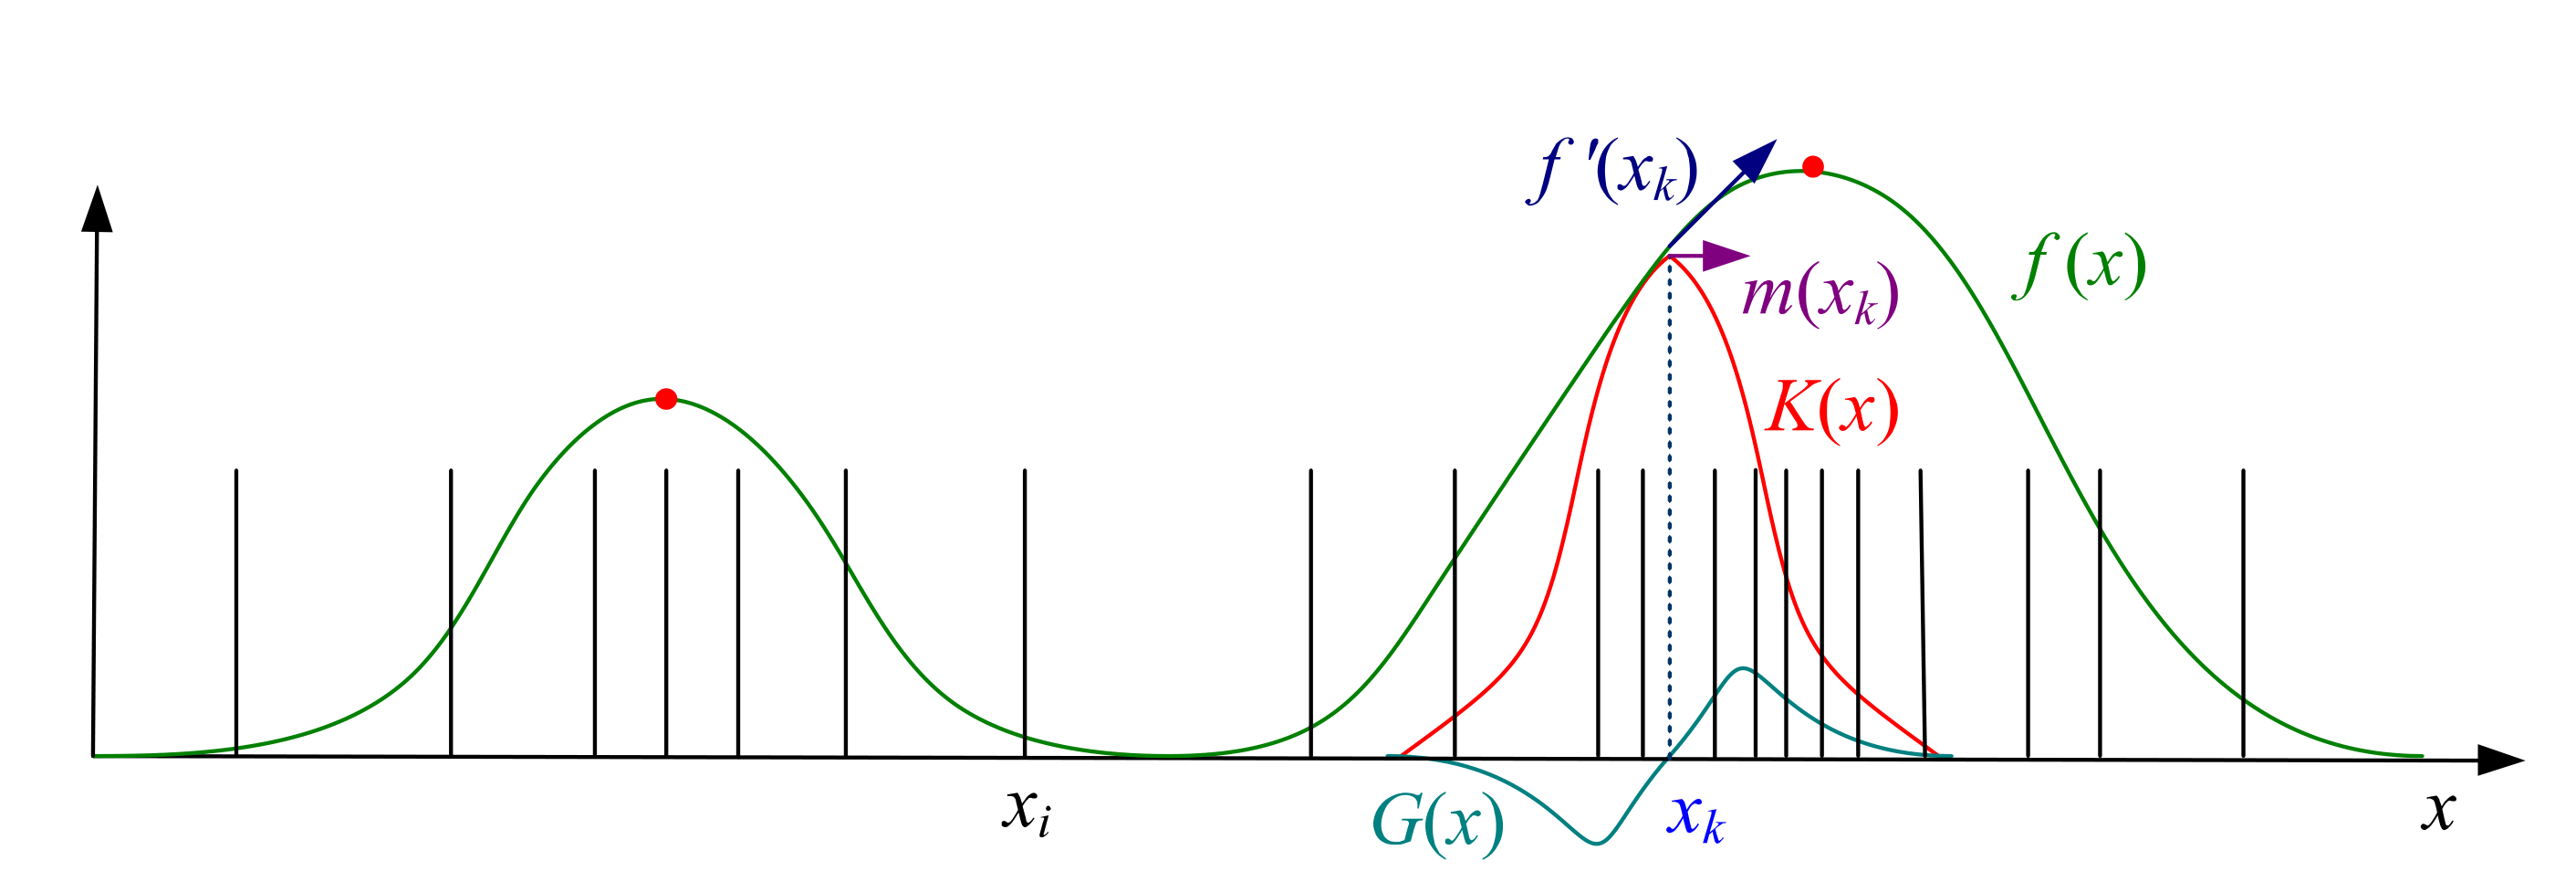
\includegraphics[width=0.7\linewidth]{img/kernel_density_estimation}
	\caption{Kernel Density Estimation}
\end{figure}

\subsubsection{Mean Shift Algorithm}

For all positions $x$ in the image, calculate the mean $\samplemean{x}$ in the environment $N(x)$:

\[
\samplemean{x} = \frac{\sum_{x_i \in N(x)} K(x_i - x) x_i}{\sum_{x_i \in N(x)} K(x_i - x)}
\]

Set $x$ to the mean $\samplemean{x}$ and iterate until $x$ does not change.
Attraction basins are regions from which all trajectories lead to the same node.

\begin{figure}[h]
	\centering
	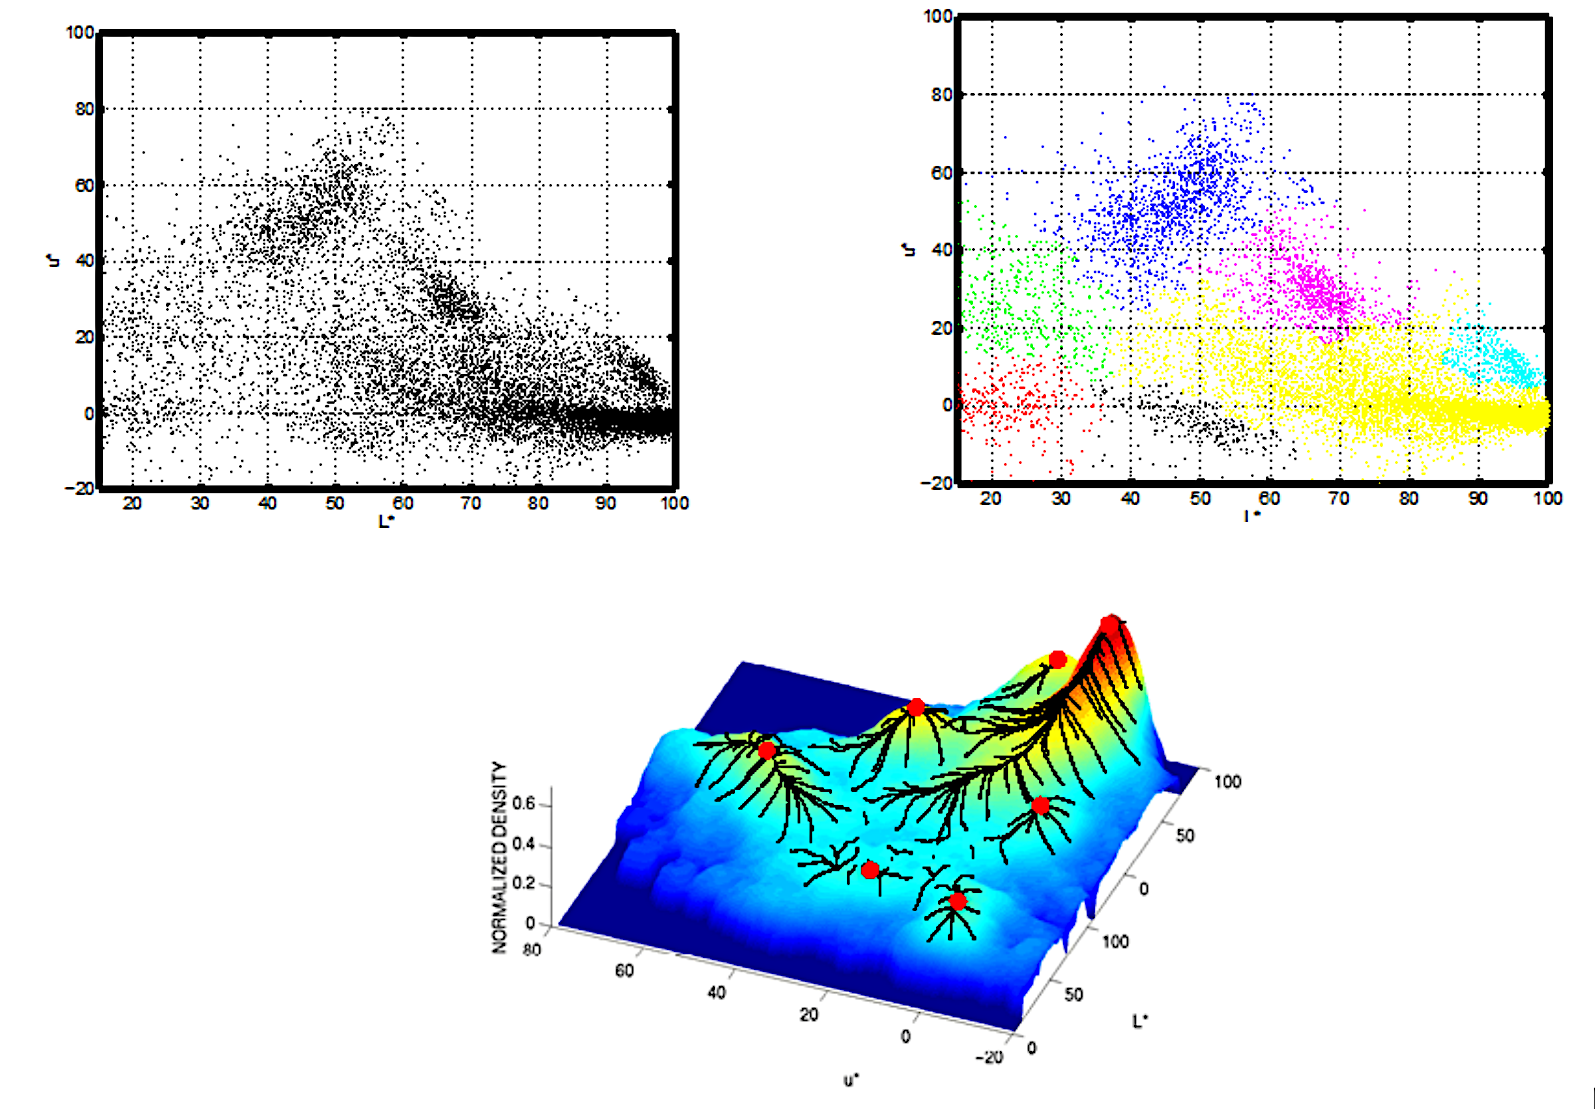
\includegraphics[width=0.7\linewidth]{img/attraction_basins}
	\caption{Attraction Basins in Mean Shift Clustering}
\end{figure}

\subsection{Segmentation by Graph Cuts}

Images are represented as graphs with nodes for pixels and edges between nodes with affinity weights.
These weights measure similarity, such as inversely proportional to the difference in color and position.

\begin{definition}
	Let $G=(V,E)$ be a graph. Each edge $(u,v)$ has a weight $w(u,v)$ representing the similarity between $u$ and $v$.
	Cut $G$ into two disjoint graphs with node sets $A$ and $B$ by removing all edges between those sets.
	Assign a value to the cut as follows:

	\[
	\text{cut}(A,B) = \sum_{u\in A,v\in B}^{w(u,v)}
	\]
\end{definition}

Minimal value cuts often lead to small groups. Normalized cuts, using $\text{Ncut}(A,B)$,
offer a better approach by considering associations and dissimilarities.

\subsection{Superpixels}

The inefficiency of graph calculations with many pixels in images is addressed by calculating \emph{superpixels}—grouping similar pixels.
This cost-effective method may lead to over-segmentation, but applying normalized graph cuts to superpixels can mitigate this issue.

\subsection{Features}

Raw input pixel values are not directly used as features to avoid a large input space.
Instead, feature vectors are calculated for each pixel or set of pixels to capture specific properties of an image or image region.
These feature vectors are crucial for various tasks, including classification, subregion detection, and image stitching.

\subsubsection{Feature Properties}

Features should be invariant to translation, rotation, scaling, illumination changes, color variations, and transformations (skewing).

\subsubsection{Filter Banks}

Filter banks, as illustrated in Figure \ref{fig:filter_bank},
consist of RFS Filters (edge and line filters at six orientations and three scales, Gaussian, and Laplacian of Gaussian)
and MR8 Filters (Maxima of RFS Filters at each scale).

\begin{figure}[h]
	\centering
	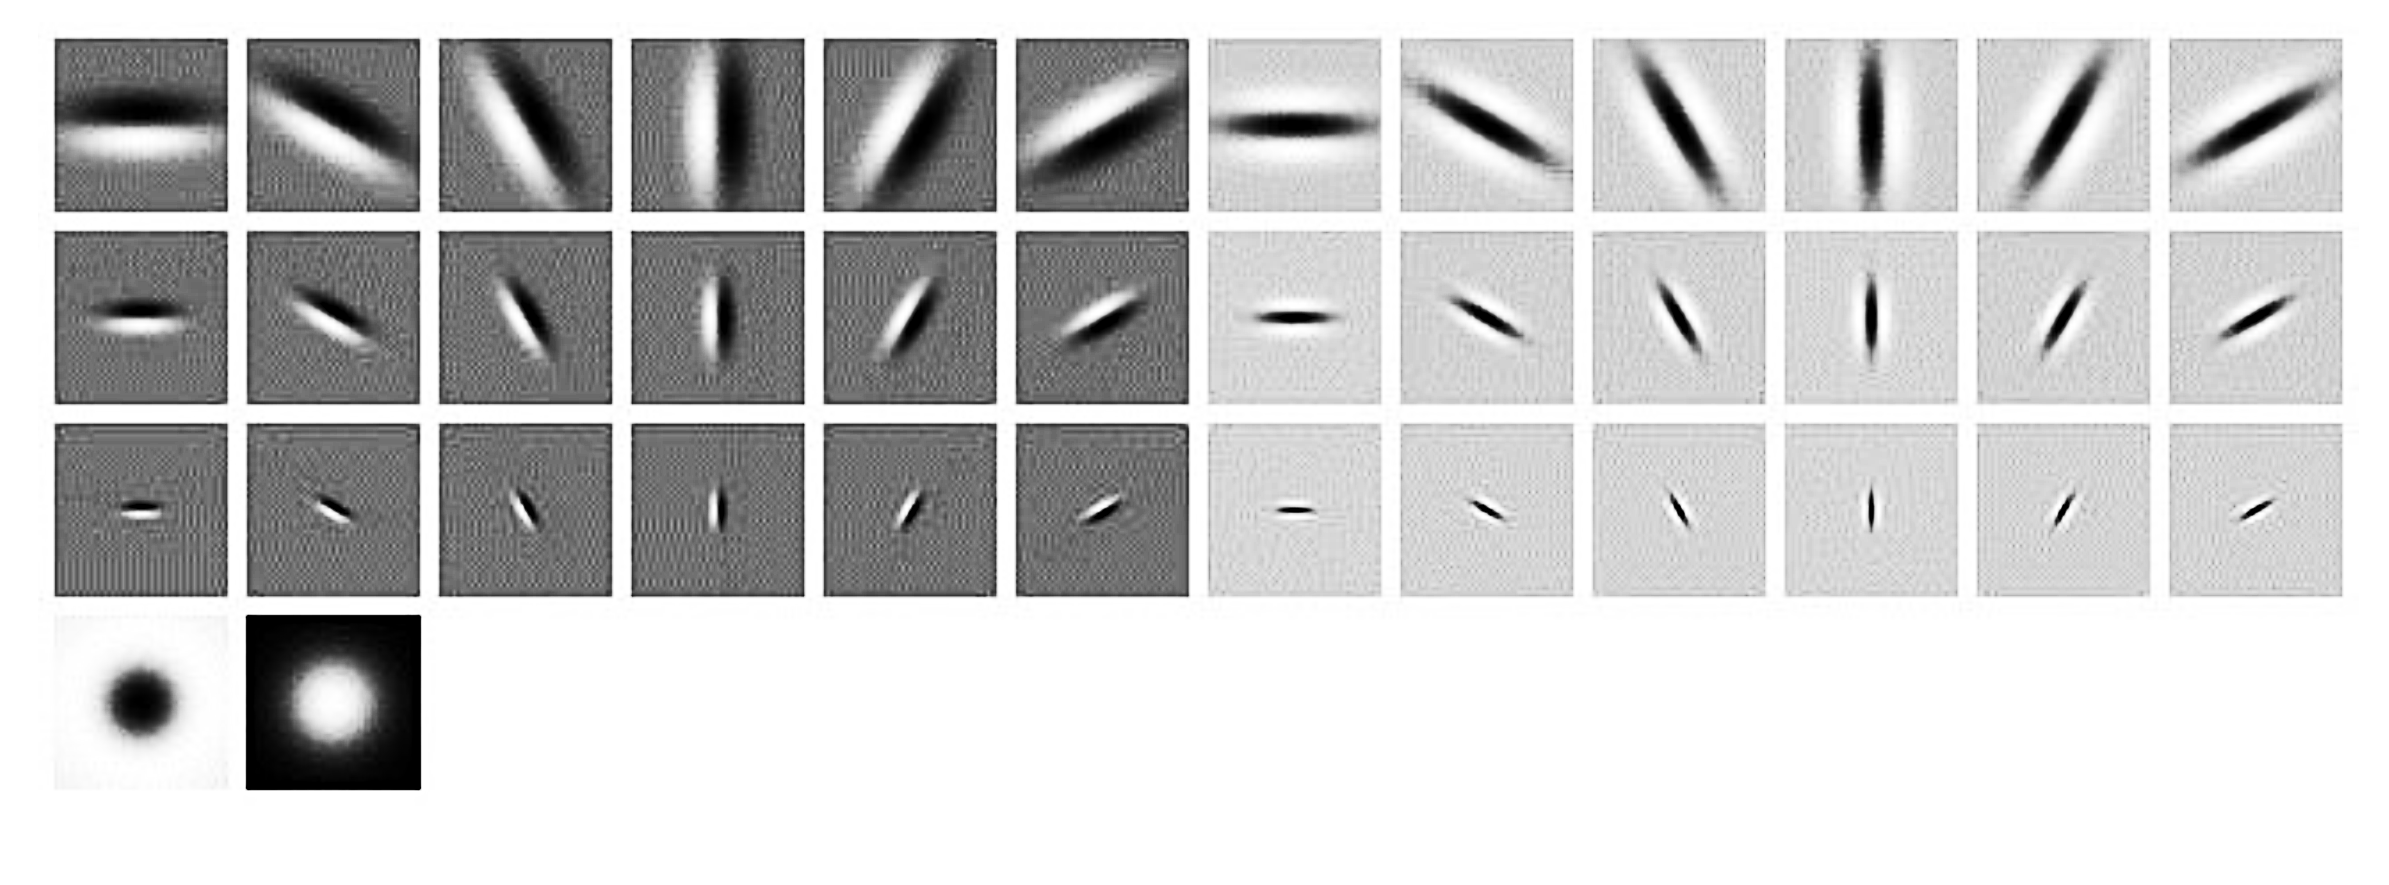
\includegraphics[width=0.6\linewidth]{img/filter_bank}
	\caption{Filter Banks}
	\label{fig:filter_bank}
\end{figure}

\subsubsection{Texture Characteristics}

Textons utilize texture descriptors as vectors of filter bank outputs. Textons obtained through clustering form a dictionary,
and the similarity between regions in the texton histograms is used for comparison.

\subsubsection{Grey Level Co-occurrence Matrices (GLCMs)}

GLCM measures how often a specific combination of color values between a pixel and its neighbors occurs.
This results in a $256\times 256$ matrix for the 256 grey values.
Additional features like entropy, energy, homogeneity, contrast, or dissimilarity can be calculated from the matrix.

\subsubsection{Scale Invariant Feature Transform (SIFT)}

SIFT is a popular feature descriptor for tasks such as object matching and image stitching.
It combines detection and description, using the histogram of the gradient and resulting in a 128-dimensional vector.

\begin{figure}[h]
	\centering
	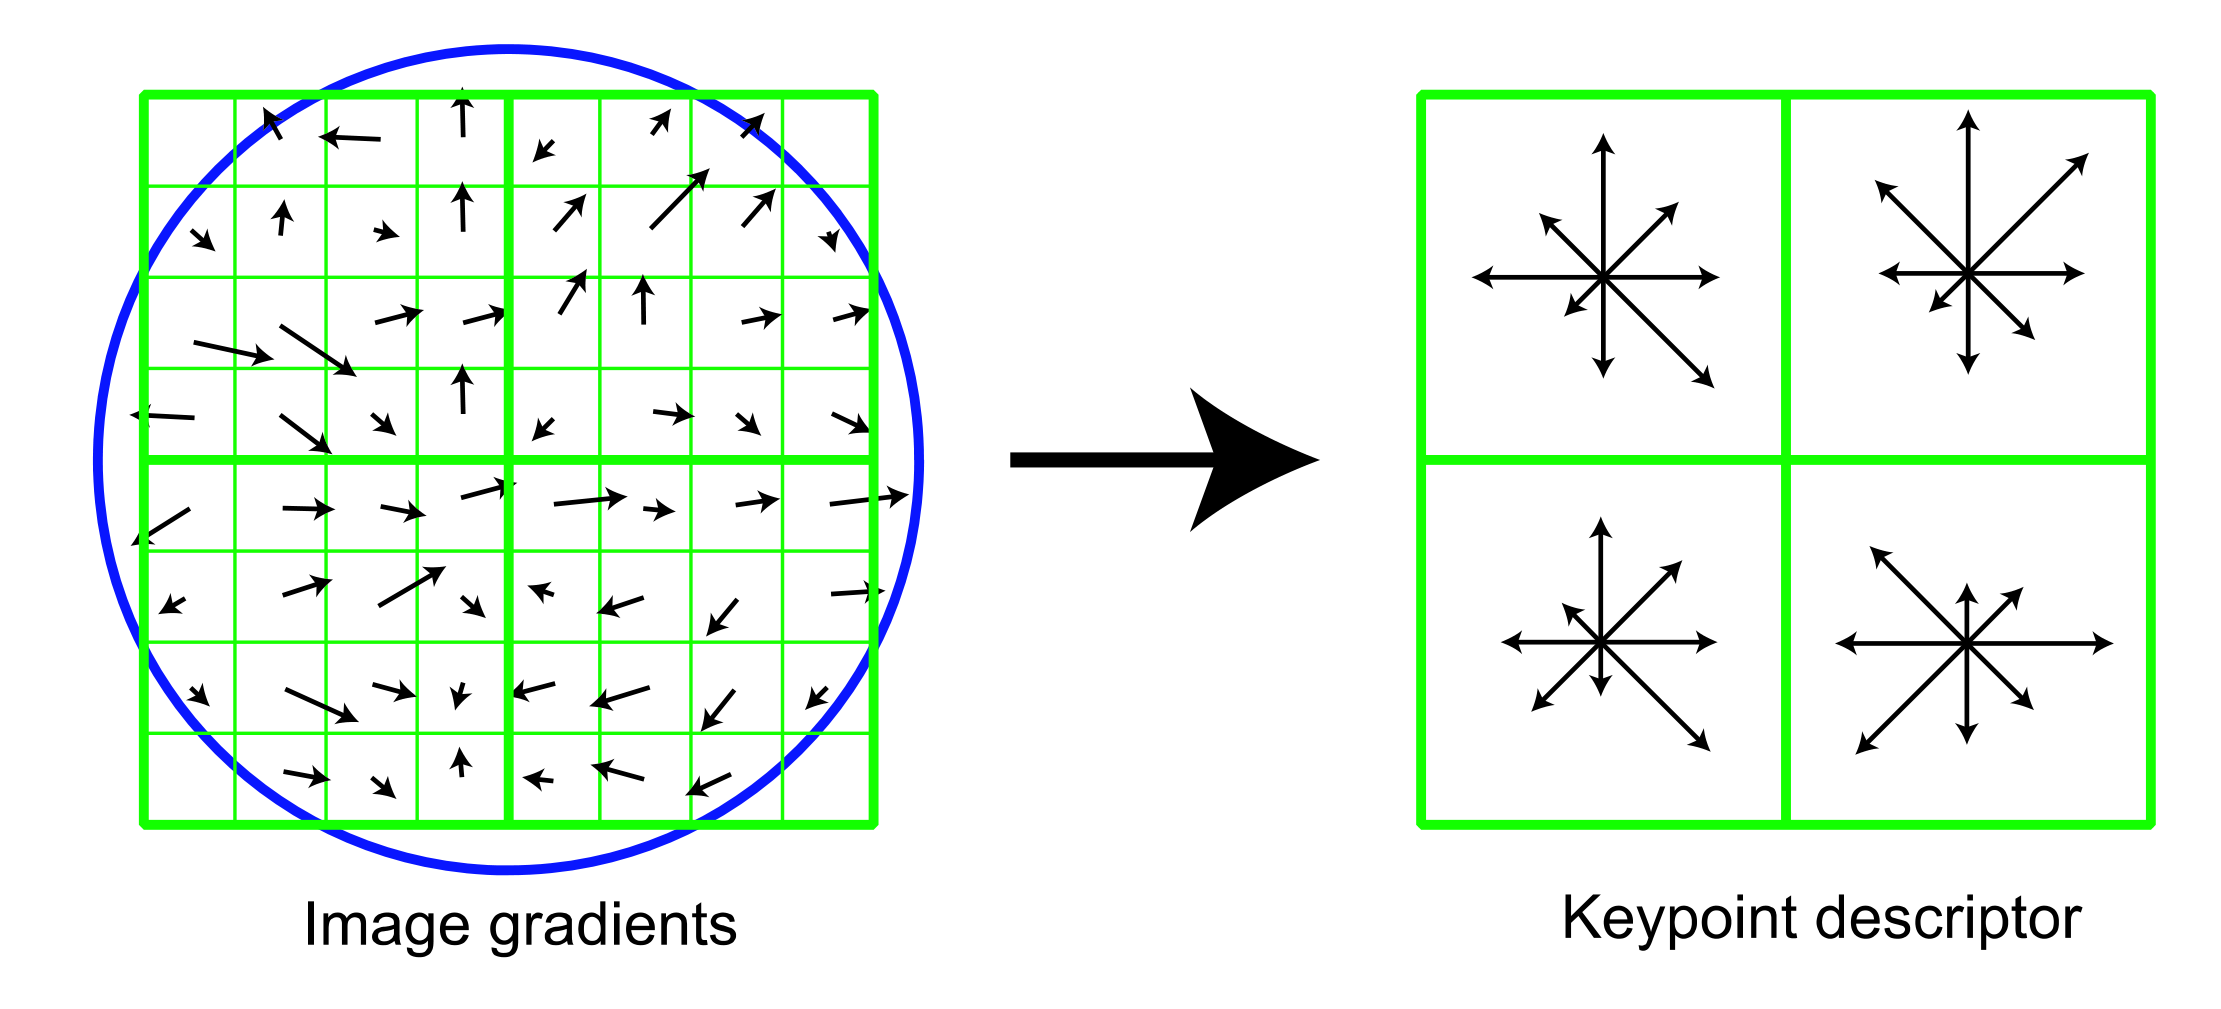
\includegraphics[width=0.6\linewidth]{img/SIFT}
	\caption{Scale Invariant Feature Transform (SIFT)}
\end{figure}

\subsubsection{Histogram of Oriented Gradients (HOG)}

HOG computes gradient images in x and y and divides the image into cells.
It then calculates the histogram of gradient orientation in each cell, normalizes, and flattens it into a feature vector.

\subsubsection{HOGles}

HOGles "inverts" HOG features to simulate the image that generates them. This tool is useful for understanding bad detections.

\begin{figure}[h]
	\centering
	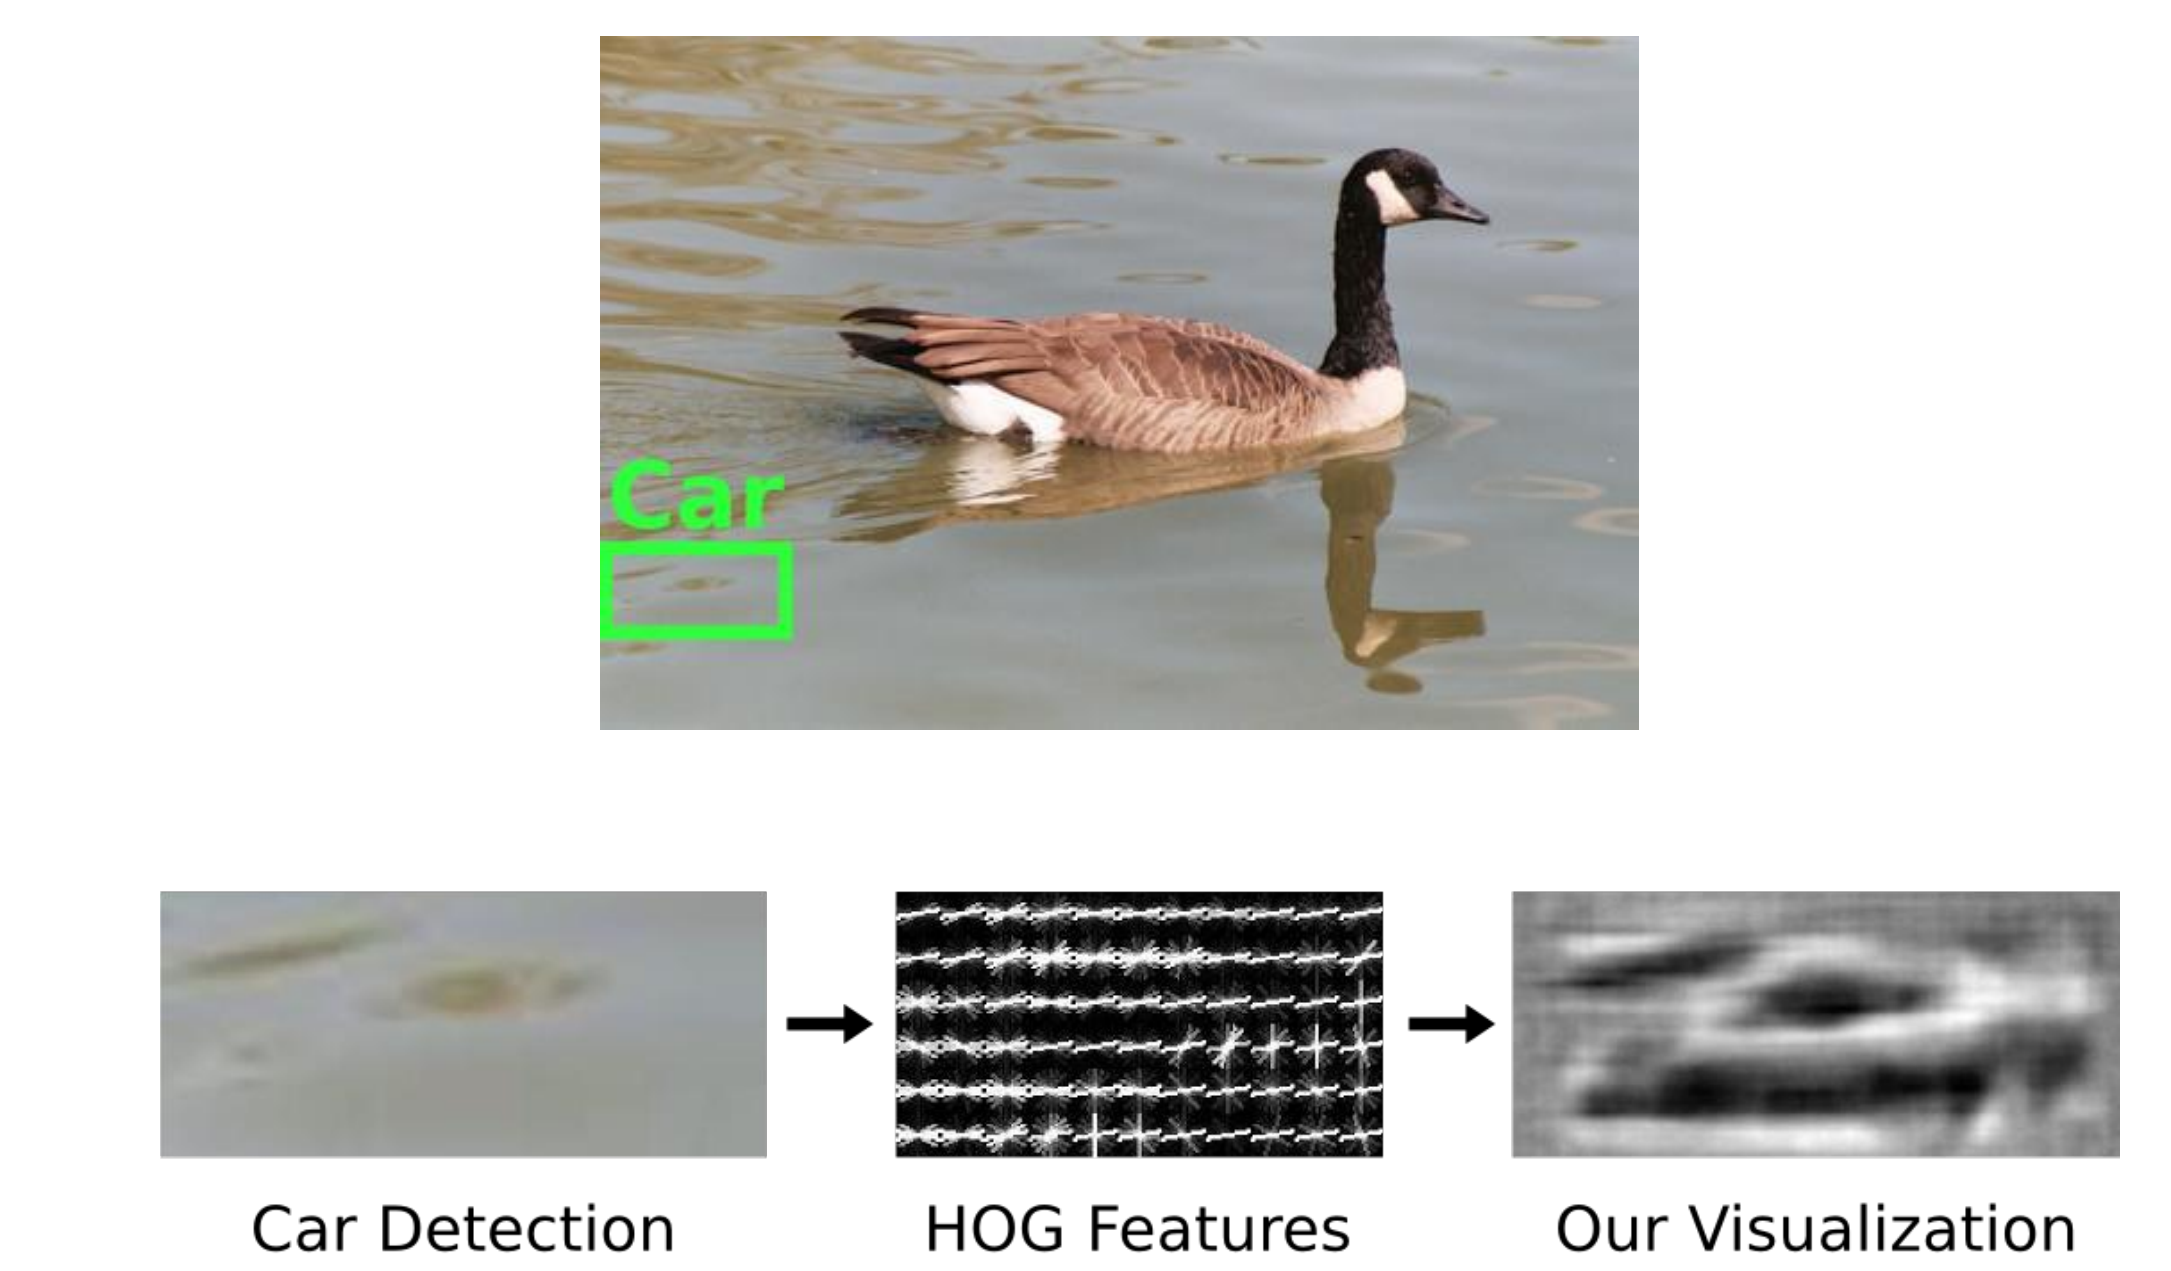
\includegraphics[width=0.6\linewidth]{img/HOGles}
	\caption{HOGles: Inverted HOG Features}
\end{figure}
